%!TEX encoding=UTF-8 Unicode
%!TEX root=../tabarnac.tex

\section{Related Work}
\label{sec:soa}

This section presents an overview of related work in the area of data mapping mechanisms and memory access profiling of parallel applications based on shared memory.

\subsection{Data Mapping Mechanisms}
\label{sec:soa-mapping}

Form a high-level view, data mapping mechanisms can be classified into two categories, mechanisms that have information about the memory access before the application starts executing, and mechanisms without prior information that need to determine the memory access behavior during execution of the parallel application.
Mechanisms that have prior information have the advantage of potentially higher improvements compared to mechanisms without prior information, as the collection of information during runtime has a potentially high overhead.
Furthermore, opportunities for improvements are lost while information about the memory access pattern is collected.
On the other hand, if the memory access behavior is analyzed during application execution, no prior analysis is required.
Figure~\ref{fig:timeline} shows a comparison of the operation of these two types of applications with a parallel application consisting of four threads.
In this example, a mechanism with prior information can perform the mapping as soon as the parallel phase starts (or even earlier), while mechanisms without this information need to learn the behavior for some time and can perform mapping decisions only at a later stage of the execution.

\begin{figure}[!b]
    % 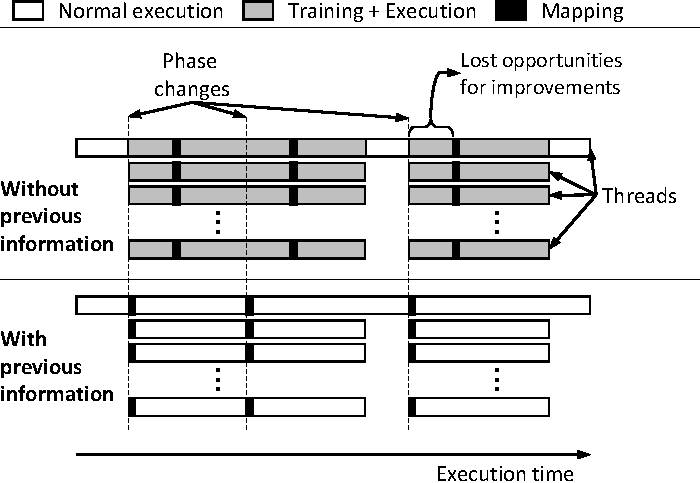
\includegraphics[width=\linewidth]{img/timeline}
    %!TEX encoding=UTF-8 Unicode
%!TEX root=../tabarnac.tex

\def\len{6}
\def\wid{0.3}
\def\dis{0.1}

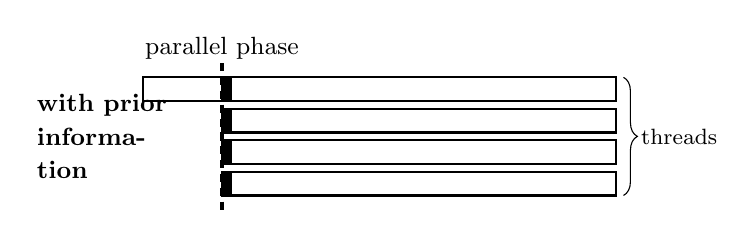
\begin{tikzpicture}
	\node[align=left, text width=1.7cm] at (-0.5,-\wid-1.5*\dis) (label1) {\bfseries\small with prior information};

	\draw[thick] (0,0)              rectangle +(\len, \wid);
	\draw[thick] (1,-\wid*0-\dis*1) rectangle +(\len-1,-\wid);
	\draw[thick] (1,-\wid*1-\dis*2) rectangle +(\len-1,-\wid);
	\draw[thick] (1,-\wid*2-\dis*3) rectangle +(\len-1,-\wid);

	\draw[fill=black] (1,0)              rectangle +(0.12,\wid);
	\draw[fill=black] (1,-\wid*0-\dis*1) rectangle +(0.12,-\wid);
	\draw[fill=black] (1,-\wid*1-\dis*2) rectangle +(0.12,-\wid);
	\draw[fill=black] (1,-\wid*2-\dis*3) rectangle +(0.12,-\wid);

	\draw[very thick,densely dashed] (1,1.6*\wid) -- +(0,-\wid*5-\dis*4.3) node[near start,pos=-0.1] {\small parallel phase};

	\draw [decorate,decoration={brace,amplitude=5pt}] (\len+.1,\wid) -- ++(0,-4*\wid-3*\dis) node [midway,right=1mm]{\footnotesize threads};

	% \draw (-1.35,-\wid*5) -- +(8.8,0); %separator


\end{tikzpicture}


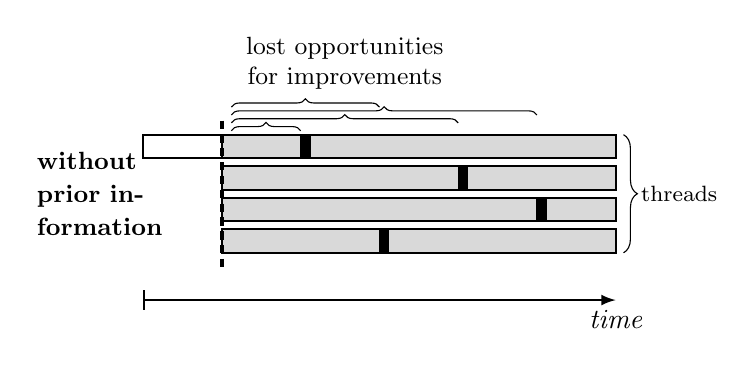
\begin{tikzpicture}
	\node[align=left, text width=2cm] at (-0.35,-\wid-1.5*\dis) (label1) {\bfseries\small without prior information};

	\draw[thick] (0,0)              rectangle +(\len, \wid);
	\draw[fill=gray!30, thick] (1,0)              rectangle +(\len-1, \wid);
	\draw[fill=gray!30, thick] (1,-\wid*0-\dis*1) rectangle +(\len-1,-\wid);
	\draw[fill=gray!30, thick] (1,-\wid*1-\dis*2) rectangle +(\len-1,-\wid);
	\draw[fill=gray!30, thick] (1,-\wid*2-\dis*3) rectangle +(\len-1,-\wid);

	\draw[fill=black] (2,0)              rectangle +(0.12,\wid);
	\draw[fill=black] (4,-\wid*0-\dis*1) rectangle +(0.12,-\wid);
	\draw[fill=black] (5,-\wid*1-\dis*2) rectangle +(0.12,-\wid);
	\draw[fill=black] (3,-\wid*2-\dis*3) rectangle +(0.12,-\wid);

	\draw[decorate,decoration={brace,amplitude=3pt}] (1+0.12,\wid+0.05) -- +(1-0.12,0);
	\draw[decorate,decoration={brace,amplitude=3pt}] (1+0.12,\wid+0.15) -- +(3-0.12,0)node[midway,above=3mm,align=center,font=\small] {\small lost opportunities\\ for improvements};
	\draw[decorate,decoration={brace,amplitude=3pt}] (1+0.12,\wid+0.25) -- +(4-0.12,0);
	\draw[decorate,decoration={brace,amplitude=3pt}] (1+0.12,\wid+0.35) -- +(2-0.12,0);

	\draw[very thick,densely dashed] (1,1.6*\wid) -- +(0,-\wid*5-\dis*4.3);

	\draw[decorate,decoration={brace,amplitude=5pt}] (\len+.1,\wid) -- ++(0,-4*\wid-3*\dis) node [midway,right=1mm]{\footnotesize threads};

	\draw[thick,|-latex] (0,-\wid*6) -- +(\len,0) node[below] {\itshape time};

\end{tikzpicture}

    \caption{Comparison of data mapping mechanisms with and without prior information about the memory access behavior of a parallel application consisting of four threads.}
    \label{fig:timeline}
\end{figure}

\subsubsection{Mechanisms Without Prior Information}

% kernel old
Most mechanisms that have no prior information about the memory access behavior operate on the operating system.
Traditionally, operating systems have used the \emph{first-touch}~\cite{Marchetti1995}, \emph{next-touch}~\cite{Lof2005} and \emph{interleave}~\cite{Kleen2004} policies to map memory pages to NUMA nodes.
The first-touch policy~\cite{Marchetti1995}, which is the default policy in most current operating systems (such as Linux), allocates a page on the NUMA node that performs the first memory access to it.
The page is never migrated between nodes.
First-touch requires that the programmer takes care of which thread accesses data first.
In some circumstances, this policy can lead to reduced performance, for example when a single thread initializes a large part of the memory and places most pages on a single node.
In next-touch~\cite{Lof2005}, each page is periodically migrated to the NUMA node that performs the next access to a page.
This policy can lead to excessive page migrations if the memory access behavior is changing fast.
The interleave policy (which is available in Linux via the \texttt{numactl} tool~\cite{Kleen2004} for example) distributes memory pages equally among all NUMA nodes, but does not take any locality of memory accesses into account.

Newer developments in operating systems focus on refining the data mapping during execution of parallel applications, using online profiling of memory accesses to guide migrations decisions.
Recent versions of the Linux kernel (starting with version 3.8) contain the NUMA Balancing technique~\cite{Corbet}, which uses page faults during execution to determine if a page should be migrated to a different NUMA node. To increase the accuracy of this mechanism, additional page faults are inserted during execution.
A similar proposal is the AutoNUMA approach~\cite{Corbet2012}.
Neither mechanism keeps an access history, eliminating the need to store the access behavior, but also making them susceptible to excessive migrations.
Other proposals keep such an access history.
Dashti et al.~\cite{Dashti2013} introduced the Carrefour mechanism, which uses instruction-based sampling~(IBS) available in recent AMD architectures~\cite{AMD2012} to detect the memory access behavior.
kMAF~\cite{Diener2014} is a similar mechanism that uses page faults to analyze the behavior.

% hardware
% marathe, lapt

\subsubsection{Mechanisms With Prior Information}

Most mechanisms with prior information about memory access behavior perform mapping in user space, on the compiler or runtime library level.
Piccoli et al.~\cite{Piccoli2014} propose a compiler extension that analyzes the memory access pattern of loops that are executed in parallel and use this information to migrate pages before the loop is entered.
Nikolopoulos et al.~\cite{Nikolopoulos2000a,Nikolopoulos2000} present an integrated compiler/OS-based data mapping mechanism based on a custom OpenMP compiler and IRIX kernel extensions. The compiler inserts instrumentation code to identify access patterns to shared memory areas, which are used to guide migration decisions.
ForestGOMP~\cite{Broquedis2010a} requires source code annotations to identify memory access behavior and is limited to the OpenMP library.

Libraries that support NUMA-aware memory allocation include libnuma~\cite{Kleen2004} and MAi~\cite{Ribeiro2009}. With these libraries, data structures can be allocated according to the specification of the programmer, such as on a particular NUMA node, or with an interleave policy. These techniques can achieve large improvements, but place the burden of the mapping on the programmer, who has to determine the best placement by hand. An evolution of MAi, the Minas framework~\cite{Ribeiro2010}, optionally uses a source code preprocessor to determine data mapping policies for arrays. Previous research also uses memory access traces to perform data mapping~\cite{Diener2015,Marathe2010,Bolosky1992}. These can be useful to determine the maximum gains that can be achieved with mapping policies, but are not applicable in general due to their substantial overhead and the fact that the access behavior might change with different input data and different numbers of threads, among others.


\subsection{Memory Access Profiling}
\label{sec:soa-profiling}

Many tools were designed to analyze and improve NUMA behavior. Nevertheless, analyzing
memory accesses is a challenge due to the amount of information to store and process.
Several tools~\cite{Lachaize12MemProf,McCurdy2010}  address this difficulty by
using sampling mechanism such as \emph{AMD  Instruction Based
Sampling}~\cite{Drongowski07Instructionbased}. Not only can sampling miss important events, leading to inaccurate characterizations, but \emph{IBS} is a non-portable \emph{AMD}
technology, therefore such tools can be used only in special circumstances. Another approach is to
use hardware performance counters~\cite{Majo13(Mis)understanding,
Jiang14Understanding,Bosch00Rivet,Weyers14Visualization,Tao01Visualizing},
which are special hardware registers that record events such as cache
misses and remote memory accesses, among others. These counters only provide a partial view
of the execution, they show events happening on the processor related to
memory, but not what triggered these events.

The second difficulty of memory analysis is to present the information in such a
 way to the user that he is able to improve the behavior. Some of the tools previously mentioned only provide
a textual output~\cite{Lachaize12MemProf,McCurdy2010}. Even if these tools highlight the most relevant informations, it is hard to get a global
view of the memory behavior from such output. The user might be lost in a
huge amount of information and not able to differentiate normal behavior from
problematic ones. Other tools provide more advanced visualizations. For
instance, Tao et al.~\cite{Tao01Visualizing} propose a detailed view for each
page, showing the number of remote and local accesses on each NUMA node. Weyers et
al.~\cite{Weyers14Visualization} present the memory bandwidth between each pair of nodes,
showing where the remote accesses occur. Finally, Bosch et al.~\cite{Bosch00Rivet} give several views of the execution and the possibility to
navigate through them.
\MD{weak paragraph...}

Although all these tools allow the user to understand more or less easily and
precisely what kind of performance issue he is facing, they never give the
reason \emph{why} a certain behavior is happening or how to improve it, which is actually the most important point that can help to fix performance issues.
Previous studies aimed to answer this question for some specific
benchmarks~\cite{Majo13(Mis)understanding,Jiang14Understanding}.
However, these studies use manual source code analysis and performance counters and do not provide a general tool or methodology usable for other applications.

\subsection{Summary}

Summarizing our discussion of previous work in this area, we can affirm that tools to improve the memory access behavior on NUMA architectures with prior information have the highest potential for improvements.
The two main challenges for this type of tool is to gather information about the memory access behavior in a fast, accurate and easy-to-use way, and providing information to the developer on how to improve the behavior.
Our proposed tool, \TABARNAC, attempts to solve these challenges.

% \MD{mechanisms with prior information have highest potential for improvements, but currently:
% - lack of information about memory access behavior
% - lack of information about ways to improve behavior
% }
% Importance of Mapping:
% \begin{itemize}
%     \item First touch
%     \item Interleave
% \end{itemize}

% Why Not automated tools
% \begin{itemize}
%     \item Trainning time
%     \item Garbage in/ garbage out (matrix modulo / bloc)
% \end{itemize}

% New tool: understand why performances are bad
